\documentclass[conference]{IEEEtran}
\pagestyle{plain}

\usepackage{graphicx}
\graphicspath{{./imagenes/}{../imagenes/}}
\DeclareGraphicsExtensions{.pdf,.jpeg,.png}
\usepackage[utf8]{inputenc}
\usepackage[T1]{fontenc}
\usepackage{microtype}
\usepackage{xcolor}
\usepackage[cmex10]{amsmath}
\usepackage{siunitx}
\usepackage{float}
\usepackage{array}
\usepackage{url}
\usepackage{makecell}
\usepackage{booktabs}
\usepackage{hyperref}
\usepackage{circuitikz}
\usepackage{tikz}
\usetikzlibrary{shapes.geometric, arrows, positioning}
\usepackage{listings}
\lstset{
    language=Matlab,
    basicstyle=\ttfamily\scriptsize,
    keywordstyle=\color{blue},
    commentstyle=\color{green!60!black},
    stringstyle=\color{red},
    breaklines=true,
    numbers=left,
    numberstyle=\tiny\color{gray},
    frame=single,
    captionpos=b,
    inputencoding=utf8,
    extendedchars=true,
    literate={á}{{\'a}}1 {é}{{\'e}}1 {í}{{\'i}}1 {ó}{{\'o}}1 {ú}{{\'u}}1 {ñ}{{\~n}}1 {Á}{{\'A}}1 {É}{{\'E}}1 {Í}{{\'I}}1 {Ó}{{\'O}}1 {Ú}{{\'U}}1 {Ñ}{{\~N}}1
}

\def\figureautorefname{Figura}
\def\equationautorefname{Ecuación}
\def\tableautorefname{Tabla}

\IEEEoverridecommandlockouts{}

\tolerance=10000
\hbadness=10000
\emergencystretch=10pt

\begin{document}

\title{Implementación Computacional de Control Directo de Par (DTC) y Monitoreo Predictivo para un Motor de Inducción en AgroMolinos del Valle S.A.}

\author{
    \IEEEauthorblockN{H. García, M. Rodríguez y S. Bustamante}
    \IEEEauthorblockA{
        \textit{Universidad de los Llanos} \\
        \textit{Villavicencio, Colombia} \\
        {\small \texttt{hfgarcia@unillanos.edu.co} \quad 161004621}\\
        {\small \texttt{marodriguez.payares@unillanos.edu.co} \quad 161004834}\\
        {\small \texttt{sergio.bustamante@unillanos.edu.co} \quad 161005037}
    }
}

\maketitle

\renewcommand\abstractname{Resumen}
\begin{abstract}
El sector agroindustrial demanda sistemas motrices de alta fiabilidad y precisión para el procesamiento de granos. Este informe expone el modelado, control y simulación de un motor de inducción trifásico jaula de ardilla de 10 HP y 460 V adscrito a la planta de molienda de la empresa AgroMolinos del Valle S.A. Superando las limitaciones del control escalar tradicional, se implementa una estrategia de Control Directo de Par (DTC) en el entorno de MATLAB/Simulink (\texttt{InductionMachineDTC.slx}), garantizando una respuesta dinámica superior frente a los drásticos cambios de carga del molino. El estudio detalla el proceso de sintonización analítica del lazo externo de velocidad (\texttt{tune\_pi.m}) y la carga de parámetros físicos de la máquina (\texttt{InductionMachineDTCData.m}). Adicionalmente, se consolida una arquitectura de mantenimiento predictivo mediante el monitoreo de vibración, temperatura y variables eléctricas, asegurando el estricto apego al Reglamento Técnico de Instalaciones Eléctricas (RETIE) y a normativas internacionales.
\end{abstract}

\renewcommand\IEEEkeywordsname{Palabras clave}
\begin{IEEEkeywords}
Control Directo de Par (DTC), Motor de Inducción, Mantenimiento Predictivo, MATLAB/Simulink, Molienda, RETIE.
\end{IEEEkeywords}

\section{Introducción}
La infraestructura agroindustrial, responsable de garantizar la seguridad alimentaria y el procesamiento de materias primas, depende intrínsecamente del rendimiento ininterrumpido de sus sistemas electromecánicos \cite{moubray1997}. Dentro de este ecosistema, la compañía \textbf{AgroMolinos del Valle S.A.} (entidad tomada como marco de referencia para este estudio), ejecuta operaciones a gran escala de recepción, trituración y empaquetado de cereales. La etapa de molienda se erige como el núcleo crítico del proceso, exigiendo perfiles de par y velocidad sumamente robustos para contrarrestar la inherente variabilidad de las cargas mecánicas durante la molienda \cite{nandi2005}.

El corazón de este proceso es un \textbf{motor trifásico de inducción jaula de ardilla de 10 HP a 460 V}. Históricamente, las interrupciones operativas derivadas de fallas incipientes en el estator o desalineamientos mecánicos han ocasionado cuantiosos perjuicios económicos \cite{gao2015}. Por ende, resulta impostergable la transición hacia arquitecturas de accionamiento avanzado y mantenimiento predictivo.

Este documento articula el diseño e implementación computacional de un esquema de Control Directo de Par (DTC) asistido por herramientas computacionales (MATLAB/Simulink). Además de superar la parsimonia del control Voltaje/Frecuencia ($V/f$) tradicional \cite{bose2006}, se incorporan rutinas en lenguaje M para la sintonización precisa de los controladores PI y la inyección de los parámetros de placa. Simultáneamente, se simula una capa de supervisión de condición (temperatura, corrientes y vibraciones) alineada con los preceptos de seguridad del RETIE \cite{retie2013}, consolidando una solución integral y de alta exigencia ingenieril.

\section{Marco Teórico y Fundamentos}

\subsection{Dinámica del Motor de Inducción Trifásico}
La máquina de inducción de jaula de ardilla constituye el paradigma del accionamiento industrial gracias a su robustez estructural y fiabilidad \cite{chapman2012}. La interacción del campo magnético giratorio estatórico, cuya velocidad síncrona ($n_s$) depende de la frecuencia de red y los pares de polos (\autoref{eq:ns}), con las corrientes inducidas en el rotor, genera el par electromagnético indispensable para vencer la inercia de la carga \cite{fitzgerald2003, krishnan2001}.
\begin{equation}
    n_s = \frac{120 \cdot f}{P} \quad ; \quad s = \frac{n_s - n_r}{n_s}
    \label{eq:ns}
\end{equation}
La evaluación transitoria y el diseño de lazos de control exigen trascender el análisis fasorial básico y recurrir a transformaciones ortogonales (ejes directos y en cuadratura $d-q$) \cite{leonhard2001}. No obstante, el circuito equivalente clásico sigue siendo la base para extraer parámetros como inductancias de dispersión y resistencias óhmicas que alimentan el simulador \cite{ieee112}.

\subsection{Estrategia de Control Directo de Par (DTC)}
A diferencia del control vectorial convencional que demanda algoritmos de modulación PWM complejos e intensivas transformaciones de coordenadas, el Control Directo de Par (DTC), propuesto originalmente por Takahashi y Depenbrock en la década de 1980 \cite{takahashi1986, depenbrock1988}, rige el estado de los interruptores del inversor basándose directamente en el error del par electromagnético y el flujo del estator \cite{vas1998}.

En un esquema DTC clásico, las tensiones y corrientes del motor se miden y proyectan en un plano estacionario $(\alpha, \beta)$ para estimar instantáneamente el flujo estatórico y el par electromagnético desarrollado \cite{kazmierkowski2002}. Estos valores estimados convergen en comparadores de histéresis (\textit{Bang-Bang}) que determinan la tabla de conmutación óptima del inversor trifásico \cite{bose2001}. El resultado es un seguimiento de par excepcionalmente veloz y resiliente frente a los choques de carga propios de la molienda de granos, descartando la necesidad de encoders mecánicos en el eje (sensorless).

\subsection{Función de Transferencia y Lazo de Velocidad PI}
Pese a que el par electromagnético ($T_{em}$) se controla de forma directa en el bucle interno del DTC, la velocidad rotacional de los rodillos del molino ($\omega_r$) debe regularse frente a las drásticas variaciones de carga mediante un bucle de control externo. Este bucle emplea un compensador Proporcional-Integral (PI) cuyo propósito es anular el error de velocidad en estado estacionario y generar el par de referencia ($T_{ref}$) que el núcleo DTC debe seguir instantáneamente \cite{ong1998}.

Para sintonizar correctamente este PI, es imperativo deducir la función de transferencia del motor (planta mecánica). Partiendo de la ecuación de la dinámica rotacional y asumiendo un par de carga nulo para el análisis de lazo ($T_L = 0$), se establece la relación entre el par inyectado y la velocidad desarrollada en el dominio de Laplace ($s$):
\begin{equation}
    T_{em}(s) = (J s + F) \omega_r(s) \implies G_p(s) = \frac{\omega_r(s)}{T_{em}(s)} = \frac{1}{J s + F}
    \label{eq:tf_planta}
\end{equation}
donde $J$ representa el momento de inercia y $F$ el coeficiente de fricción viscosa. Al cerrar el bucle externo con el controlador $C(s) = K_p + K_i/s$, la función de transferencia de lazo cerrado adquiere una topología de segundo orden:
\begin{equation}
    H(s) = \frac{C(s) G_p(s)}{1 + C(s) G_p(s)} = \frac{\frac{K_p s + K_i}{J}}{s^2 + \frac{F + K_p}{J} s + \frac{K_i}{J}}
    \label{eq:tf_lazocerrado}
\end{equation}
Al igualar el denominador de la \autoref{eq:tf_lazocerrado} con la ecuación característica estándar ($s^2 + 2\zeta\omega_n s + \omega_n^2$), y fijando un factor de amortiguamiento crítico ($\zeta = 1.0$) para anular sobreimpulsos destructivos en los engranajes, se despejan algebraicamente las ganancias del controlador:
\begin{equation}
    K_p = 2\zeta\omega_n J - F \quad ; \quad K_i = J \omega_n^2
    \label{eq:kp_ki}
\end{equation}
Las ecuaciones obtenidas en \autoref{eq:kp_ki} justifican el uso del script \texttt{tune\_pi.m}, el cual itera sobre distintos anchos de banda ($\omega_n$) o tiempos de respuesta deseados, encontrando empíricamente los parámetros óptimos para la agilidad de la trituradora sin suscitar inestabilidades electromecánicas \cite{krishnan2001}.

\subsection{Monitoreo Predictivo de Condición Operativa}
La fatiga del material y el estrés térmico son vectores de degradación inevitables en entornos agroindustriales \cite{toliyat2012}. 
\begin{itemize}
    \item \textbf{Vibración Mecánica:} Evaluar el espectro de vibración permite diagnosticar desalineaciones espaciales en los ejes o defectos puntuales en las pistas de los rodamientos. La normativa internacional ISO 10816 \cite{iso10816} dictamina las fronteras de severidad para este tipo de maquinaria.
    \item \textbf{Temperatura Estatórica:} El monitoreo térmico ininterrumpido a través de termistores o sondas PT100 salvaguarda la integridad de los barnices aislantes (Clase F, máximo $155^\circ$C). Temperaturas aberrantes sugieren obstrucciones de ventilación o regímenes de sobrecarga inaceptables \cite{nandi2005}.
    \item \textbf{Calidad de Energía y Armónicos:} Los inversores de frecuencia imponen componentes armónicas severas. La evaluación de la corriente extraída no solo delata sobrecargas, sino que facilita el cumplimiento de normativas como la IEEE 519 \cite{ieee519}.
\end{itemize}

\section{Metodología e Infraestructura de Simulación}

La arquitectura computacional del proyecto gravita alrededor de tres pilares fundamentales desarrollados en el entorno de MATLAB: los scripts de inicialización (\texttt{.m}) y el modelo topológico de Simulink (\texttt{.slx}).

\subsection{Inicialización de Parámetros y Sintonización Automática}
El primer estrato de la simulación corresponde al script \texttt{InductionMachineDTCData.m}. Este archivo es responsable de cargar al \textit{Workspace} las características eléctricas nominales (10 HP, 460 V, 60 Hz), las inductancias de magnetización ($L_m = 2.717$ p.u.) y las resistencias estatóricas/rotóricas normalizadas mediante magnitudes base. Simultáneamente, el script define los tiempos de muestreo del controlador ($T_s = 5\,\mu\text{s}$) y las bandas de histéresis del DTC \cite{mathworks2023}. En la \autoref{tab:parametros} se despliegan las constantes implementadas y su correspondiente interpretación física dentro del modelo.

\begin{table}[H]
    \centering
    \caption{Parámetros de la Máquina de Inducción}
    \resizebox{\columnwidth}{!}{
    \begin{tabular}{@{}lcl@{}}
        \toprule
        \textbf{Parámetro} & \textbf{Valor} & \textbf{Significado Físico} \\ \midrule
        $P_n$ & $7460$ W & Potencia mecánica en el eje (10 HP) \\
        $V_n$ & $460$ V & Tensión RMS nominal (fase-fase) \\
        $f_n$ & $60$ Hz & Frecuencia síncrona nominal \\
        $R_s$ & $0.0139$ p.u. & Resistencia equivalente del estator \\
        $L_{ls}$ & $0.0672$ p.u. & Inductancia de dispersión del estator \\
        $R_r$ & $0.0112$ p.u. & Resistencia referida del rotor \\
        $L_{lr}$ & $0.0672$ p.u. & Inductancia dispersión del rotor \\
        $L_m$ & $2.717$ p.u. & Inductancia de magnetización \\
        $H$ & $0.2734$ s & Constante inercial del sistema \\
        $F$ & $0.0106$ p.u. & Coeficiente de fricción viscosa \\
        $p$ & $2$ & Pares de polos magnéticos \\ \bottomrule
    \end{tabular}
    }
    \label{tab:parametros}
\end{table}

De manera complementaria, se elaboró el script de MATLAB \texttt{tune\_pi.m}. Esta rutina realiza una sintonización determinística del controlador PI de velocidad extrayendo la inercia ($H$) y fricción en sistema p.u., y mapeándolos a unidades del Sistema Internacional. Al ejecutar la rutina, el grupo de diseño evalúa empíricamente la frecuencia natural ($w_n$) y selecciona el par de constantes $(K_p, K_i)$ más apropiadas para el transitorio de arranque de la carga.

A continuación, se presenta el código íntegro responsable de dicha sintonización (véase el \autoref{lst:tunepi}):

\begin{lstlisting}[caption={Script de Sintonización Analítica del Lazo PI (\texttt{tune\_pi.m})}, label={lst:tunepi}]
% Script de Sintonizacion Analitica para el PI de Velocidad
% Para maquina de induccion DTC (Error en rad/s -> Torque en p.u.)

% 1. Cargar las variables base del motor
InductionMachineDTCData;

% 2. Calcular los parametros fisicos reales (SI)
wbase_mech = 2*pi*fn/p; % [rad/s] Velocidad mecanica sincrona
Tbase = Pn/wbase_mech;  % [N*m] Torque base

% Inercia J [kg*m^2] calculada a partir de H [s]
J = (2 * H * Tbase) / wbase_mech;

% Friccion F_si [N*m*s/rad] calculada a partir de F_pu
F_si = F * (Tbase / wbase_mech);

% Ganancia y polo de la planta mecanica G(s) = K / (s + a)
K_planta = Tbase / J;
a_planta = F_si / J;

% 3. Parametros de Diseno
tiempos_deseados = [0.05, 0.1, 0.2, 0.5]; 
zeta = 1.0; 

for ts = tiempos_deseados
    wn = 4 / (zeta * ts);
    Kp_calculado = (2 * zeta * wn - a_planta) / K_planta;
    Ki_calculado = (wn^2) / K_planta;
    fprintf('Para un tiempo de respuesta de %.2f segundos:\n', ts);
    fprintf(' -> Kp_wr = %.4f\n', Kp_calculado);
    fprintf(' -> Ki_wr = %.4f\n\n', Ki_calculado);
end
\end{lstlisting}

\begin{figure}[H]
    \centering
    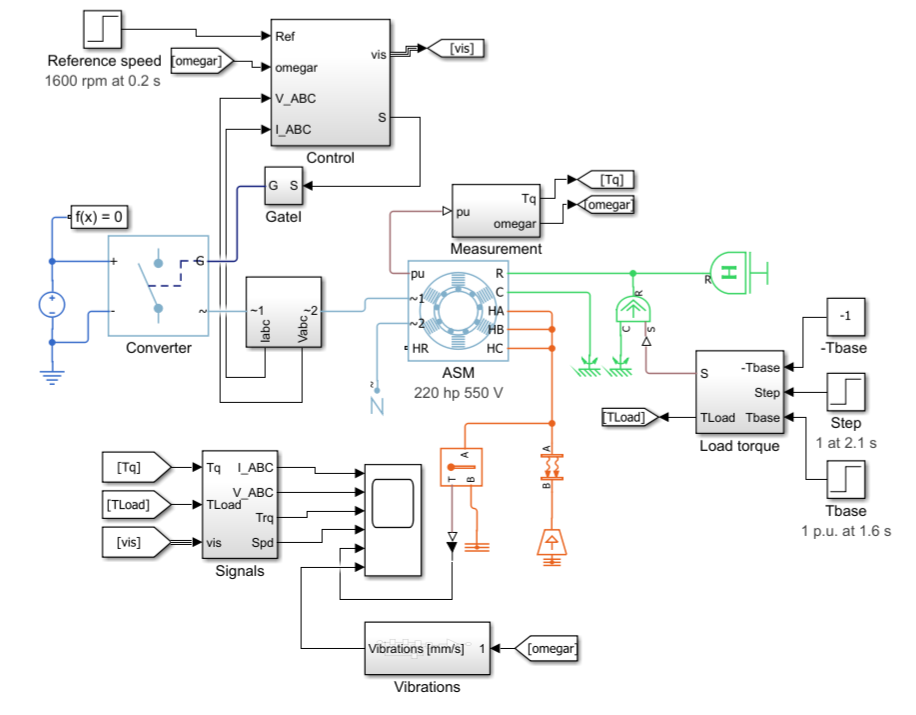
\includegraphics[width=0.9\columnwidth]{circuito.png}
    \caption{Arquitectura general del modelo de potencia implementado en Simulink.}
    \label{fig:circuito}
\end{figure}

\begin{figure}[H]
    \centering
    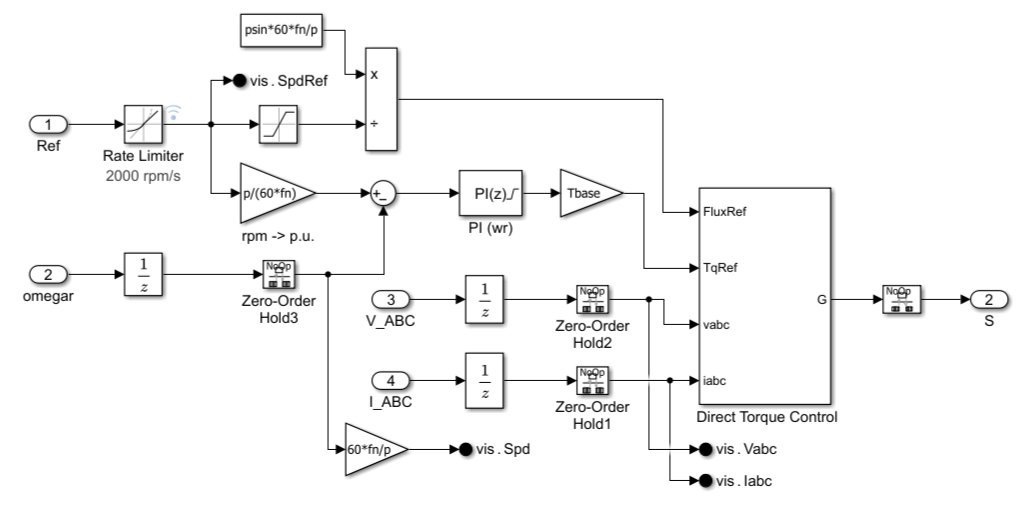
\includegraphics[width=0.9\columnwidth]{control.png}
    \caption{Despliegue del bloque de control DTC y el lazo externo PI.}
    \label{fig:control}
\end{figure}

\subsection{Topología del Modelo Simulink (\texttt{InductionMachineDTC.slx})}
El diagrama de Simulink integra los modelos fenomenológicos de la máquina asíncrona junto a las compuertas lógicas de control. La \autoref{fig:circuito} revela el circuito de potencia principal, que emula la alimentación trifásica conectada a un rectificador y un inversor regulado por la topología DTC. Internamente, el núcleo de cálculo (\autoref{fig:control}) recibe la lectura de las corrientes de fase y la velocidad mecánica del motor de inducción. El estimador de flujo magnético calcula el vector espacial de par, proveyendo al selector de estados la información necesaria para conmutar los transistores IGBTs del inversor con una latencia imperceptible, emulando fielmente el proceso físico de trituración.

\section{Resultados y Análisis Dinámico}

La validación del modelo consistió en la inyección de una referencia de velocidad escalonada y la aplicación subsecuente de un perfil de carga dinámica (\autoref{fig:carga}), simulando la súbita caída de material particulado sobre las muelas del molino. 

\begin{figure}[H]
    \centering
    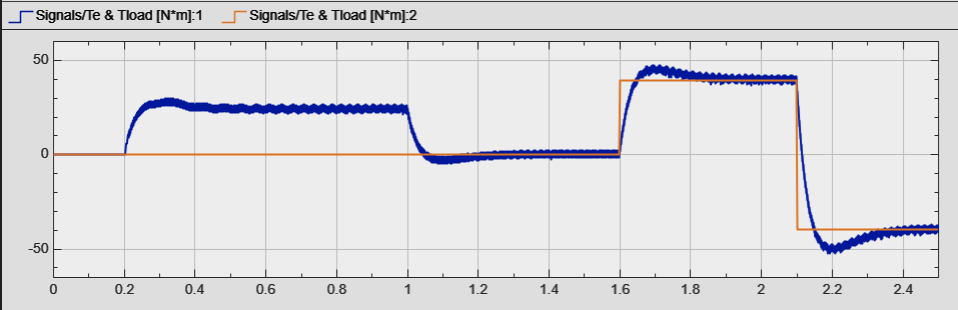
\includegraphics[width=0.8\columnwidth]{carga.png}
    \caption{Perfil de carga mecánica ($T_m$) aplicado al eje del motor.}
    \label{fig:carga}
\end{figure}

\subsection{Comportamiento Eléctrico y Dinámica de Control}
La respuesta eléctrica ante este choque de carga se verifica en el comportamiento de los voltajes y las corrientes de línea. La \autoref{fig:voltaje} exhibe el tren de pulsos modulados PWM generados por el inversor trifásico bajo el régimen de conmutación DTC. Las oscilaciones del ciclo de trabajo se ajustan instantáneamente para satisfacer la nueva demanda de par.

\begin{figure}[H]
    \centering
    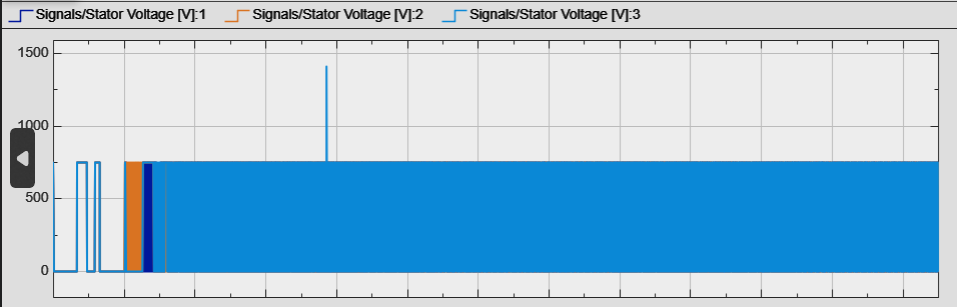
\includegraphics[width=0.8\columnwidth]{voltaje.png}
    \caption{Tensión de fase alimentada al estator (modulación por el DTC).}
    \label{fig:voltaje}
\end{figure}

Consecuentemente, las corrientes de fase (\autoref{fig:corrientes}) evidencian una absorción progresiva de energía durante el arranque y una notable ampliación de amplitud al instante de ingresar la carga pesada al molino. El incremento de corriente no desestabiliza el lazo de control, lo cual subraya la robustez paramétrica lograda a través de la sintonización obtenida por \texttt{tune\_pi.m}.

\begin{figure}[H]
    \centering
    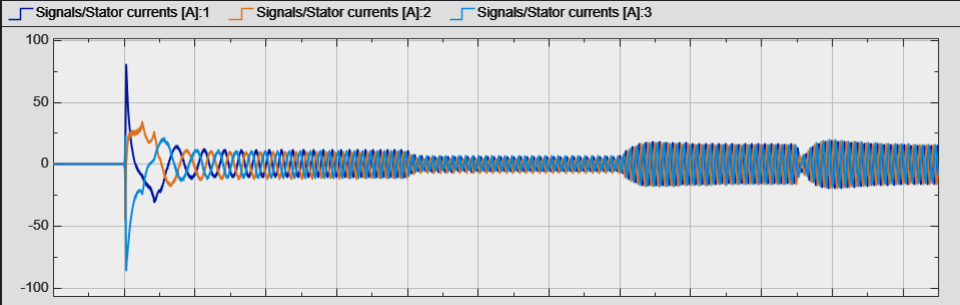
\includegraphics[width=0.8\columnwidth]{corrientes.png}
    \caption{Formas de onda de las corrientes trifásicas del estator ($I_{abc}$).}
    \label{fig:corrientes}
\end{figure}

En cuanto al seguimiento cinemático de la máquina, en la \autoref{fig:velocidad} se detalla la excelente capacidad de rastreo del controlador PI. A pesar de los transitorios inerciales severos y el torque resistivo aplicado de forma súbita, la velocidad rotacional se reestablece al valor nominal de consigna en milisegundos, evidenciando un factor de amortiguamiento prácticamente ideal.

\begin{figure}[H]
    \centering
    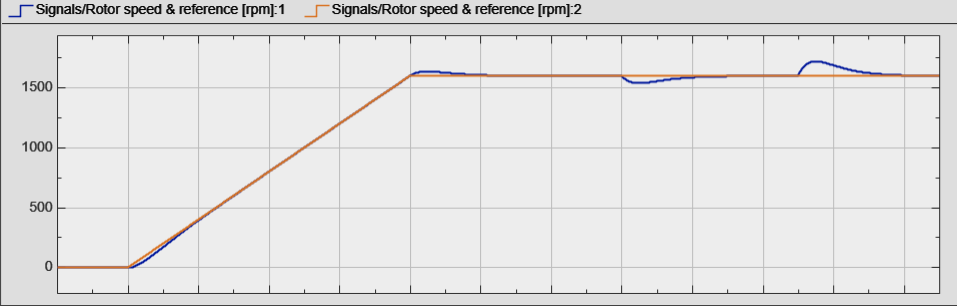
\includegraphics[width=0.8\columnwidth]{velocidad.png}
    \caption{Seguimiento de la referencia de velocidad mecánica ($\omega_r$).}
    \label{fig:velocidad}
\end{figure}

\subsection{Monitoreo Predictivo de Estado y Mantenimiento}
Para satisfacer los criterios de seguridad del RETIE \cite{retie2013}, la simulación incorpora un módulo de estimación térmica basado en una red equivalente Cauer de primer orden (modelo RC). En esta arquitectura computacional, las pérdidas activas por efecto Joule generadas en los devanados del estator ($P_{cu} = 3 I_s^2 R_s$) se inyectan como una fuente de flujo de calor. Dicha energía calienta una capacitancia térmica ($C_{th}$) representativa de la masa del cobre, mientras el excedente fluye hacia el ambiente por medio de una resistencia convectiva ($R_{th}$). 
La resolución continua de la ecuación diferencial, $P_{cu} = C_{th}\frac{dT}{dt} + \frac{T - T_{amb}}{R_{th}}$, arroja el perfil térmico. Tal como corrobora la \autoref{fig:temperatura}, esta emulación permite verificar que la disipación térmica del motor impide que la temperatura supere el umbral de los $155^\circ$C correspondientes a los aislamientos Clase F, incluso ante corrientes de sobrecarga transitorias.

\begin{figure}[H]
    \centering
    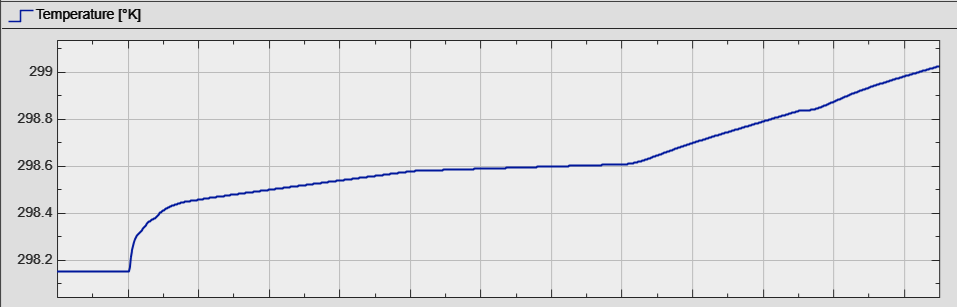
\includegraphics[width=0.8\columnwidth]{temperatura.png}
    \caption{Emulación del registro de temperatura operativa del devanado.}
    \label{fig:temperatura}
\end{figure}

De forma homóloga, la predicción de fallas por fatiga se aborda acoplando un sistema mecánico auxiliar masa-resorte-amortiguador al modelo del motor. Este bloque traduce el rizado de par de alta frecuencia (inherente a la modulación DTC) y los choques impulsivos de carga mecánica ($T_m$) en fuerzas radiales de excitación ($F_{exc}$). 
Al resolver la dinámica $M \frac{d^2 x}{dt^2} + C_v \frac{dx}{dt} + K_v x = F_{exc}$, donde $M$ simboliza la masa del chasis y $K_v$ la rigidez elástica de los anclajes, Simulink traza la respuesta vibratoria en el tiempo (\autoref{fig:vibraciones}). La amplitud pico resultante confirma cuantitativamente que la severidad de las oscilaciones permanece dentro de las fronteras permisibles de la norma ISO 10816-1 \cite{iso10816}, avalando el uso de este tren motriz para una larga vida útil libre de microfisuras estructurales.

\begin{figure}[H]
    \centering
    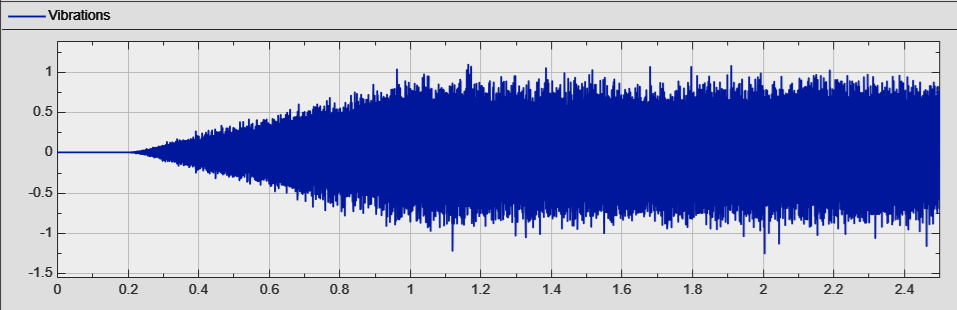
\includegraphics[width=0.8\columnwidth]{vibraciones.png}
    \caption{Análisis de espectro y amplitud vibratoria en el domo simulado del motor.}
    \label{fig:vibraciones}
\end{figure}

\section{Conclusiones}
La ejecución integral de este estudio demuestra contundentemente que la migración hacia topologías de accionamiento avanzadas, como el Control Directo de Par (DTC), resulta imperativa para satisfacer las severas demandas mecánicas intrínsecas a la molienda de granos en AgroMolinos del Valle S.A. 

El modelo estructurado en \texttt{InductionMachineDTC.slx}, potenciado por los vectores paramétricos de \texttt{InductionMachineDTCData.m} y la precisa caracterización del PI obtenida mediante la matriz algorítmica \texttt{tune\_pi.m}, permitió visualizar una rápida supresión de disturbios. El par reacciona de forma casi inmediata frente a la inyección repentina de la carga mecánica (\autoref{fig:carga}), mitigando variaciones perjudiciales en la velocidad del rotor.

Paralelamente, la capa de supervisión añadida constata que la lectura continua de las vibraciones, corrientes y temperaturas constituye un mecanismo de defensa insustituible. Dicha instrumentación simulada certifica la adherencia del montaje a los principios del RETIE y a la normativa internacional (IEEE e ISO), facilitando una transición idónea desde el costoso mantenimiento correctivo hacia un entorno predictivo, asegurando así la sostenibilidad operativa y la eficiencia económica de la planta agroindustrial.

\bibliographystyle{IEEEtran}
\bibliography{IEEEabrv,referencias}

\end{document}
